\section{Topic models and Inference}
\label{sec:models}

% Topic models discover patterns of word usage in a corpus.  Related
% words often appear in similar documents, and topic models can discover
% clusters of words that share context.  Because words in these clusters
% often seem to ``make sense'' together, they are described as topics.
% For illustration, three topics from a topic model called latent
% Dirichlet allocation (LDA)~\cite{blei-03} are shown in
% Figure~\ref{fig:nyttopics:topic}.

% Topic models are unsupervised; they do not require labels or
% annotations.  Instead, they discover latent topics directly from the
% data.  In addition to finding topics, topic models also assign
% mixtures of these topics to documents.  This is illustrated in
% Figure~\ref{fig:nyttopics:doc}. 

% We restrict ourselves to exchangeable topic models, in which the order
% of the words within a document does not matter.  The models we
% consider are also probabilistic, in the sense that they seek to
% approximate the vector of observed word counts as a mixture of topic
% distributions; fitting one of these topic models entails finding a
% point on the topic simplex that best describes the document.

Topic models posit that each document is expressed as a mixture of
topics.  These topic proportions are drawn once per document, and the
topics are shared across the corpus.  In this paper we consider Latent
Dirichlet allocation (LDA)~\cite{blei-03} a topic model which treats
each document's topic assignment as a multinomial random variable
drawn from a symmetric Dirichlet and logistic normal prior,
respectively.

Inference algorithms for all of these topic models build the same type
of latent space: a collection of topics for the corpus and a
collection of topic proportions for each of its documents.  While this
common latent space has explored for over two decades, its
interpretability remains unmeasured.

\begin{figure*}[t]
\centering
\subfigure[Topics]{
  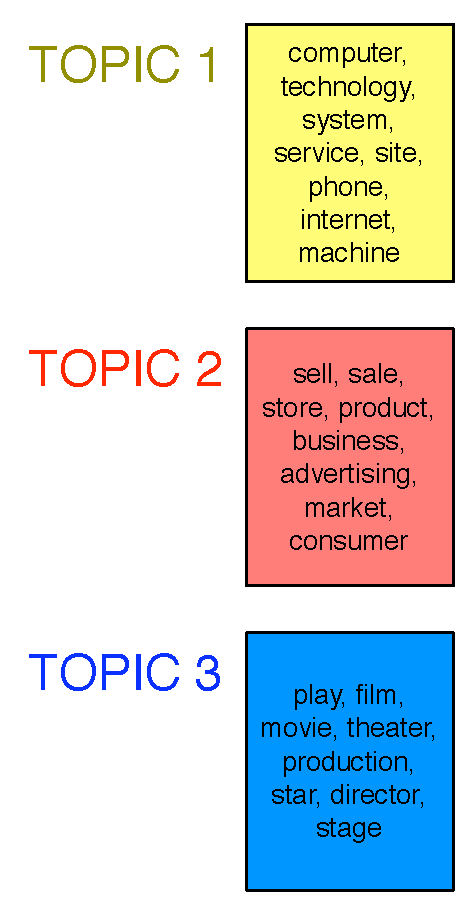
\includegraphics[scale=0.35]{figures/nyt_topics.pdf}
  \label{fig:nyttopics:topic}
}
\hspace{0.4in}
\subfigure[Document Assignments to Topics]{
  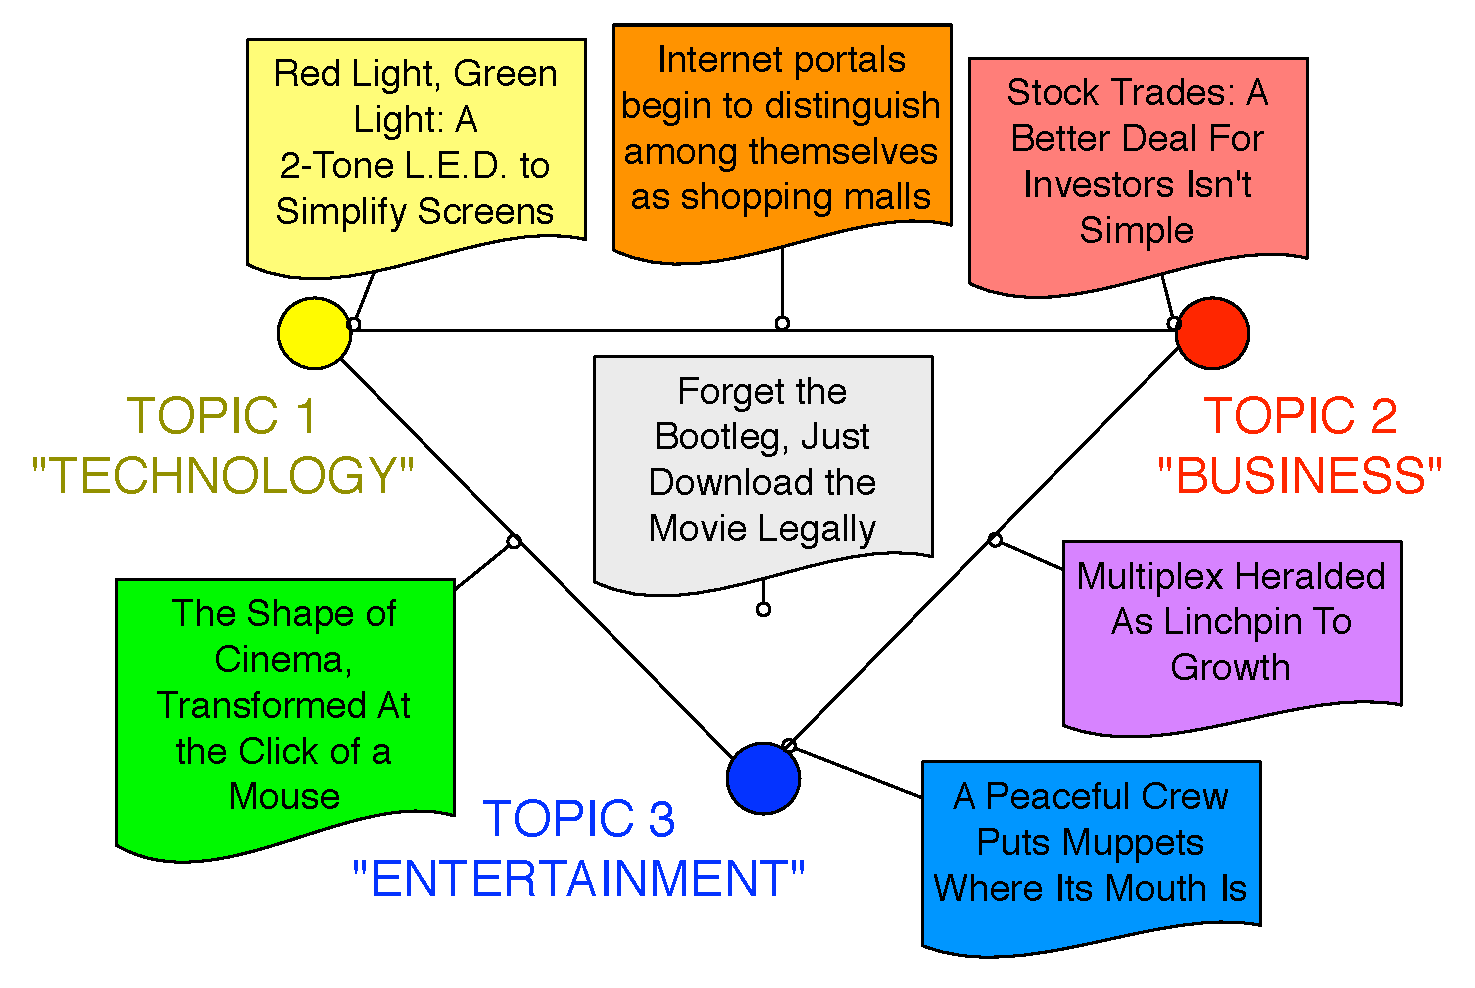
\includegraphics[scale=0.35]{figures/nyt_documents.pdf}
  \label{fig:nyttopics:doc}
}
\caption{The latent space of a topic model consists of topics,
  which are distributions over words, and a distribution over these
  topics for each document.  On the left are three topics from a
  fifty topic LDA model trained on articles from the New York
  Times.  On the right is a simplex depicting the distribution
  over topics associated with seven documents.  The line from each
  document's title shows the document's position in the topic
  space.}
\label{fig:nyttopics:big}
\end{figure*}

\begin{figure}[t]
\centering
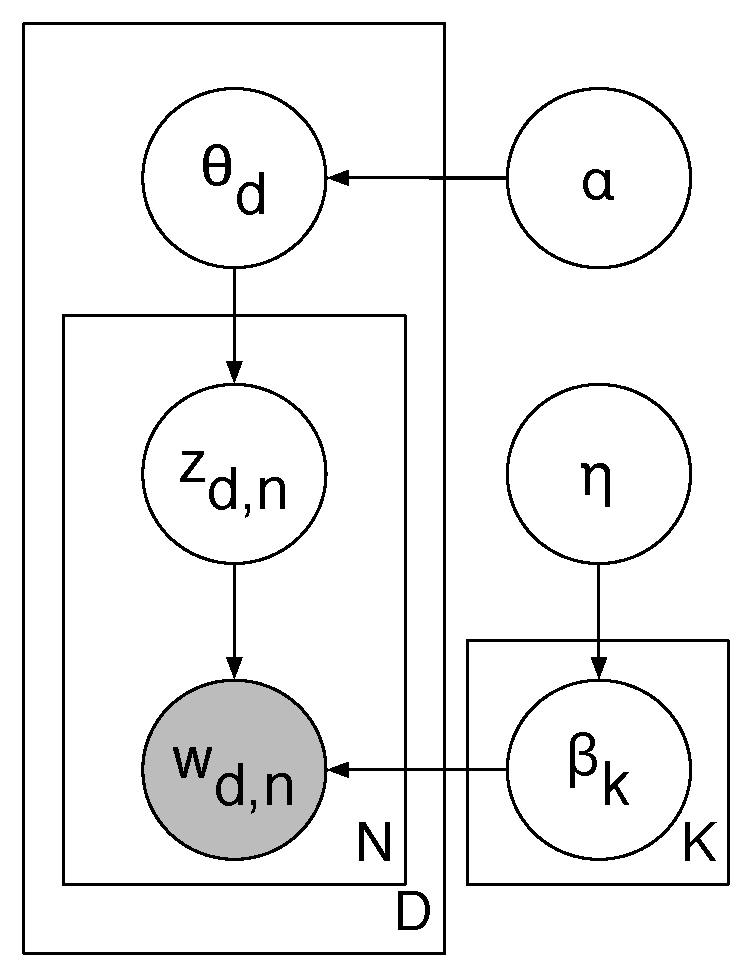
\includegraphics[width=0.5\linewidth]{figures/lda}
\caption{A graphical model depiction of latent Dirichlet allocation
  (LDA).  Plates denote replication.  Shaded circles denote observed
  variables and unshaded circles denote hidden variables.}
\label{fig:lda}
\end{figure}

Formally, the generative process of LDA is as follows:
\begin{enumerate*}
  \item For each topic $k$, 
    \begin{enumerate*}
    \item Draw topic $\beta_k \sim \mathrm{Dir}(\eta)$
    \end{enumerate*}
  \item For each document $d$, 
    \begin{enumerate*}
    \item Draw topic proportions $\theta_d \sim \mathrm{Dir}(\alpha)$
    \item For each word $w_{d, n}$, 
      \begin{enumerate*}
      \item Draw topic assignment $z_{d,n} \sim \mathrm{Mult}(\theta_d)$
      \item Draw word $w_{d,n} \sim \mathrm{Mult}(\beta_{z_{d,n}})$
      \end{enumerate*}
    \end{enumerate*}
\end{enumerate*}
The parameters of the model are the number of topics, $K$, as well as
the Dirichlet priors on the topic-word distributions and
document-topic distributions, $\alpha$ and $\eta$.  The only observed
variables of the model are the words, $w_{d,n}$.  The remaining
variables must be inferred.

There are several techniques for performing posterior inference,
i.e., inferring the distribution over hidden variables given a
collection of documents, including variational
inference~\cite{blei-03} and Gibbs sampling~\cite{griffiths-06}.  In
the sequel, we focus on the latter approach.  

Collapsed Gibbs sampling for LDA treats the topic-word and
document-topic distributions, $\theta_d$ and $\beta_k$, as nuisance
variables to be marginalized out. The posterior distribution over the
remaining latent variables, the topic assignments $z_{d,n}$, can be
expressed as
\begin{eqnarray*}
  &&p(\bm{z} | \alpha, \eta, \bm{w}) \propto \\
  &&\qquad \prod_{d}\prod_{k} \left[ \Gamma(n_{d,k} + \alpha_{k})\frac{\Gamma(\eta_{w_{d,n}} + n_{w_{d,n}, k})}{\Gamma(\sum_w n_{w, k} + \eta_w)}\right],
\end{eqnarray*}
where $n_{d,k}$ denotes the number of words in document $d$ assigned
to topic $k$ and $n_{w,k}$ the number of times word $w$ is assigned to
topic $k$.  This leads to the sampling equations,
\begin{eqnarray}
  &&p(z_{d,i} = k | \alpha, \eta, \bm{w}, \bm{z}y) \propto \\
  &&\qquad (n^{\lnot d,i}_{d,k} + \alpha_{k})\frac{\eta_{w_{d,i}} + n^{\lnot d,i}_{w_{d,i}, k}}{\sum_w n^{\lnot d,i}_{w, k} + \eta_w},
  \label{eq:sampling}
\end{eqnarray}
where the superscript $\lnot d,i$ indicates that these statistics
should exclude the current variable under consideration, $z_{d,i}$.

In essence, the model performs inference by looking at each word in
succession, and probabilistically assigning it to a topic according to
\myeq{eq:sampling}.  \myeq{eq:sampling} is derived through the
modeling assumptions and choice of parameters.  Now the question is,
when humans are given a similar assignment, to assign words to
clusters, will their own sampling equations follow \myeq{eq:sampling}
or will they be different, reflecting different underlying assumptions
about the data.

For models that use held-out likelihood, Wallach et
al.~\cite{wallach-09} provide a summary of evaluation
techniques. These metrics borrow tools from the language modeling
community to measure how well the information learned from a corpus
applies to unseen documents.  These metrics generalize easily and
allow for likelihood-based comparisons of different models or
selection of model parameters such as the number of topics.  However,
this adaptability comes at a cost: these methods only measure the
probability of observations; the internal representation of the models
is ignored.

Griffiths et al.~\cite{griffiths-06} is an important exception to the
trend of using external tasks or held-out likelihood.  They showed
that the number of topics a word appears in correlates with how many
distinct senses it has and reproduced many of the metrics used in the
psychological community based on human performance.  However, this is
still not a deep analysis of the structure of the latent space, as it
does not examine the structure of the topics themselves.

We emphasize that not measuring the internal representation of topic
models is at odds with their presentation and development.  Most topic
modeling papers display qualitative assessments of the inferred topics
or simply assert that topics are semantically meaningful, and
practitioners use topics for model checking during the development
process.  This implicit notion that topics have semantic meaning for
users has even motivated work that attempts to automatically label
topics~\cite{mei-07}.  Our goal is to measure the success of
interpreting topic models across number of topics and modeling
assumptions.
